\section{Background}
It is expected that in the future, the physical and digital worlds will merge into a largely connected globe. This is backed by the emergence of notions such as Cyber-Physical-System (CPS). 
%At the moment, CPS technologies have been applied in a broad range fo domains, including smart grids, smart homes, smart health, intelligent transportation, etc. 
CPS harbour the potential for vast economic and societal impact in domains such as automotive, health care, home automation, etc. At the same time, if these systems fail, they may cause harm and lead to temporary collapse of important infrastructures, with catastrophic consequences for industry and society. 
Therefore, in order to realise the full potential for innovation of CPS, it is important to ensure the dependability of CPS.
% - especially in relation to security and safety, as security and safety are important aspects in CPS, breaches to any of them can cause catastrophic events.

CPS are typically loosely connected and come together as temporary configurations of smaller systems which dissolve and give place to other configurations. Therefore, the configurations a CPS may assume over its lifetime are unknown and potentially infinite. Thus, currently available approaches are not possible to assure the dependability of CPS and it is a grand technology challenge to address the dependability of CPS. 

The DEIS project identifies this challenge and takes a first step towards dependability assurance of CPS by focusing on system safety and security, because assuring safety of CPS is an indispensable prerequisite in order to realise their economic and social potential.

The key innovation in the approach of the DEIS project is the concept of Digital Dependability Identity (DDI), which was outlined by key partners of DEIS in \cite{}. 
In general, a Digital Identity (DI) is defined as \emph{the data that uniquely describes a person or a thing and contains information about the subject's relationships} \cite{}. 
To this extent, a DI contains all attributes that characterise an object, how the object can be accessed, who can access it, and how it may interact with other objects. Based on this, a Digital Dependability Identity (DDI) contains all the information that uniquely describes the dependability characteristics of a CPS or a CPS component. This includes two key aspects: (a) attributes that describe the system’s or component’s dependability behaviour, such as faults and possible fault propagations through the CPS architecture, which can be described using concepts from the theory of safety contracts; and (b) requirements on how the component interacts with other entities in a dependable way, described in terms of the level of trust and assurance.

A DDI is therefore an evolution of current modular dependability assurance models for systems. It is produced during design, issued when the component is released, and then continuously maintained over the complete lifetime of a component or system. DDIs are used for the integration of components into systems during development as well as for the dynamic integration of systems into \emph{systems of systems} in the field. 
%The main difference in the two cases lies mainly in the degree of automation that integration of DDIs requires: for instance, while a manual process might be sufficient to ensure dependability requirements are met at the integration interface between silicon providers and first-tier suppliers, the dynamic integration of systems of systems in the field requires a fully automated evaluation of DDIs in order to ensure a dependable collaboration.

Based on the concept of DDI, the DEIS project seeks to provide a modelling and integration framework that lays the foundation for assuring the dependability of CPS. 




%\begin{figure}[ht!]
%	\centering
%	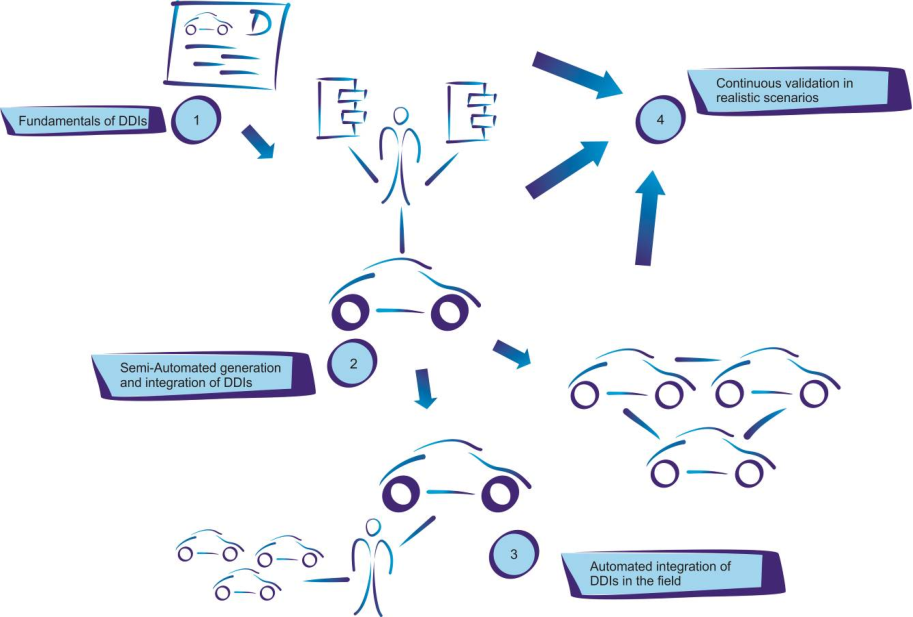
\includegraphics[width=1\linewidth]{./fig/proj_concept.pdf}
%	\caption{DEIS project concept}
%	\label{fig:proj_concept}
%\end{figure}




